\documentclass[a4paper,12pt]{report}

\usepackage[utf8]{inputenc}
\usepackage[polish]{babel}
\usepackage[MeX]{polski}
\usepackage{graphicx}
\usepackage{indentfirst}
\usepackage{multirow}
\usepackage{longtable}
\usepackage{caption}
\usepackage{multicol}
\usepackage{hhline}
\usepackage{array}
\usepackage{threeparttable}

\frenchspacing
\renewcommand\thesection{\arabic{section}.}
\renewcommand\thesubsection{\arabic{section}.\arabic{subsection}.}
\renewcommand\thesubsubsection{\arabic{section}.\arabic{subsection}.\arabic{subsubsection}.}
\brokenpenalty=5000
\clubpenalty=5000
\widowpenalty=5000
\hyphenpenalty=1000
\tolerance=300

\newenvironment{my_itemize}{
\begin{itemize}
  \setlength{\itemsep}{2pt}
  \setlength{\parskip}{0pt}
  \setlength{\parsep}{0pt}
}{\end{itemize}}


\begin{document}

% Strona tytułowa
%\maketitle
\begin{table}[!ht]
	\begin{center}
		\begin{tabular}{lcr}
		\multirow{3}{*}{\includegraphics[width=30mm]{images/logo1.png}} &
		
		\vspace{5mm}
		
		\textbf{Politechnika Gdańska} &
		\multirow{3}{*}{\includegraphics[width=25mm]{images/logo2.png}}\\
		& \textbf{WYDZIAŁ ELEKTRONIKI} & \\
		& \textbf{TELEKOMUNIKACJI I INFORMATYKI} &
		\end{tabular}
	\end{center}
\end{table}

\vspace{15mm}

\begin{par}
	\centering
		\textbf{\large{
				Dokumentacja projektu dyplomowego inżynierskiego
		}}
		
		\vspace{10mm}
		
		\emph{\textbf{\Huge{
				Edytor do proceduralnego generowania modeli drzew
		}}}
	
	
	\vspace{15mm}
	
	\begin{table}[!ht]
		\begin{center}
			\begin{tabular}{lc}
				Łukasz Odzioba & 119415 \\
				Mariusz Okrój & 119416 
			\end{tabular}
		\end{center}
	\end{table}
\end{par}

\begin{par}
	Opiekun pracy: \\
	dr inż. Michał Małafiejski

	\vspace{5mm}

	Katedra opiekuna pracy: \\
	Katedra Algorytmów i Modelowania Systemów

	\vspace{15mm}

	Streszczenie dokumentu: \\
	Dokument zawiera opis narzędzia do łatwego tworzenia trójwymiarowych modeli
	drzew w oparciu o zadany przez użytkownika zbiór parametrów opisujących oczekiwany wygląd modelu.
\end{par}

\begin{par}
	\begin{center}
		Gdańsk, 2011
	\end{center}
\end{par}

% Oświadczenie o samodzielności wykonania pracy
\newpage
\begin{par}
	\begin{center}
		\large
		\underline{OŚWIADCZENIE}
	\end{center}
\end{par}

\begin{par}
	Oświadczam, że niniejszą pracę dyplomową wykonałem samodzielnie. Wszystkie
	informacje umieszczone w~pracy uzyskane ze źródeł pisanych oraz informacje ustne
	pochodzące od innych osób zostały udokumentowane w~wykazie literatury
	odpowiednimi odnośnikami.
\end{par}

\vspace{20mm}


\begin{par}
	\begin{flushright}
		\ldots\ldots\ldots\ldots\ldots\ldots\ldots\ldots \\
		podpis dyplomanta
	\end{flushright}
\end{par}

% Spis treści
\tableofcontents

% Treść pracy
\chapter{Wstęp}

\section{Cel pracy}
Celem niniejszego projektu inżynierskiego jest stworzenie narzędzia pozwalającego na łatwe 
tworzenie trójwymiarowych modeli drzew. Narzędzie ma być przeznaczone dla osób zajmujących
się grafiką komputerową.

Ręczne modelowanie skomplikowanej struktury drzew jest bardzo czasochłonne,
dlatego też tworzenie modeli przy użyciu naszej aplikacji ma być przede wszystkim łatwe i szybkie.
W idealnym przypadku stworzenie prostego modelu drzewa możliwe byłoby w kilkanaście sekund. Ponieważ większość
grafików komputerowych posiada swój ulubiony program do pracy, nasza aplikacja powinna zapewnić
łatwy sposób na przeniesienie wygenerowanego modelu do innych narzędzi, nawet tych jeszcze nie istniejących.
Dzięki temu utworzony model może być poddany dalszej obróbce, przy pomocy bardziej zaawansowanych narzędz. Wszystko po to, aby uzyskać
efekt bliższy oczekiwaniom użytkownika.
\\ \indent Narzędzie może znaleźć zastosowanie podczas tworzenia gier, animacji, wizualizacji architektonicznych, map trójwymiarowych a nawet w celach dydaktycznych.


\newpage
\section{Funkcjonalność}
Narzędzie ma pozwalać na łatwe tworzenie trójwymiarowych modeli drzew, które następnie mogą być zapisane
w formacie obsługiwanym przez program Blender. Tworzenie modelu ma przebiegać w dwóch etapach:
\begin{itemize}
	\item{Automatyczne wygenerowanie modelu na podstawie parametrół ustalonych przez użytkownika}
	\begin{itemize}
		\item{kształt drzewa}
		\item{liczba gałęzi}
	\end{itemize}
	\item{Ręczna edycja wygenerowanego modelu przy pomocy narzędzi wbudowanych w aplikację}
	\begin{itemize}
		\item{usuwanie  i wygładzanie gałęzi}
		\item{zmiana liczby liści}
		\item{wybór tekstur kory i liści}
	\end{itemize}

	\item{Eksport do formatu obsługiwanego przez program Blender}
\end{itemize}
Bardziej szczegółowy opis wymagań znajduje się w rozdziale 2.

\section{Zadania do wykonania i podział pracy}
W tabeli poniżej zebrano najważniejsze zadania do wykonania wraz z ich podziałem na osoby odpowiedzialne
za wykonanie poszczególnych etapów.
\begin{center}    
    \begin{longtable}{|p{120mm}|p{16mm}|} \hline
    Algorytm kolonizacji przestrzeni & ŁO \\ \hline
    Zapis i odczyt ustawień programu z pliku  & ŁO \\ \hline
    Teksturowanie modelu drzewa & ŁO \\ \hline
    Eksport modelu do formatu wspieranego przez program Blender & ŁO \\ \hline
    \hline
    Tworzenie geometrii drzewa & MO \\ \hline
    Obrys korony drzewa tworzony na podstawie brył & MO \\ \hline
    Edytor do obróbki wygenerowanego modelu  & MO \\ \hline
    Rozmieszczenie liści na drzewie & MO \\ \hline
    \hline
    Opracowanie literatury & ŁO MO  \\  \hline
    Interfejs użytkownika & ŁO MO \\ \hline
    Renderowanie modelu drzewa & ŁO MO \\ \hline
    Stworzenie przykładowych modeli drzew & ŁO MO \\ \hline
    \end{longtable}
\end{center}

\section{Harmonogram}
Wstępny harmonogram prac został ustalony na początku tworzenia projektu. W trakcie pracy ulegał częstym modyfikacjom, a końcowy uproszony harmonogram przedstawia tabela umieszczona poniżej. Prace nad mniejszymi fragmentami
tworzonego systemu trwały w czasie całego okresu tworzenia, i nie zostały zawarte w tabeli. 
\\\indent Wszystkie etapy podzielono na trzy fazy, w ramach których zadania do wykonania zostały posortowane
po czasie ich rozpoczęcia, a następnie zakończenia.\\ \\
    \indent Faza analizy i projektowania
	\begin{longtable}{|p{85mm}|p{42mm}|} \hline
	

    Zapoznanie się z istniejącymi narzędziami do generowania drzew &
    1.10.2011 -- 7.10.2011
    
    \\ \hline
    Wybranie algorytmów generowania drzewa do implementacji&
    1.10.2011 -- 7.10.2011
    \\ \hline

    Opracowanie literatury&
    1.10.2011 -- 31.10.2011
    \\ \hline

    Specyfikacja wymagań funkcjonalnych&
    15.10.2011 -- 25.10.2011
    \\ \hline
    
    Projektowanie interfejsu użytkownika &
    15.10.2011 -- 1.11.2011
    \\ \hline

    Wybór formatu eksportu modelu &
    7.11.2011 -- 14.11.2011
        \\ \hline

    
    \end{longtable}
	
     Faza implementacji
    \begin{longtable}{|p{85mm}|p{42mm}|} \hline
    Implementacja algorytmu kolonizacyjnego &
    8.10.2011 -- 15.10.2011
    \\ \hline

    Implementacja algorytmów tworzenia geometrii drzewa &
    16.10.2011 -- 31.11.2011 
    \\ \hline

    Implementacja renederowania modelu drzewa &
    16.10.2011 -- 31.11.2011
    \\ \hline

    Implmentacja interfejsu użytkownika &
    1.11.2011 -- 30.11.2011
    \\ \hline

    Implementacja edytora modelu &
    15.11.2011 -- 30.11.2011
    \\ \hline

    Implementacja eksportu modelu do formatu .OBJ&
    15.11.2011 -- 30.11.2011
    \\ \hline
	
   
    
    \end{longtable}
	
    Faza wykończeniowa
    \begin{longtable}{|p{85mm}|p{42mm}|} \hline
    Testowanie aplikacji
    & 1.12.2011 -- 7.12.2011
    \\ \hline

    Przygotowanie przykładowych modeli drzew
    & 1.12.2011 -- 7.12.2011
    \\ \hline
	
    Opracowanie dokumentacji projektu
    & 1.11.2011 -- 7.12.2011
    \\ \hline
	
    \end{longtable}


\chapter{Specyfikacja wymagań}
Użytkownikiem aplikacji mają być osoby posiadające podstawową wiedzę dotyczącą grafiki trójwymiarowej,
chcące łatwo i szybko stworzyć model drzewa i wykorzystać go do swoich celów. Z powyższego założenia
wynika istotna kwestia, mianowicie obsługa narzędzia musi być prosta i intuicyjna. \\

\section{Wymagania funkcjonalne} 
Poniżej zebrano wymagania funkcjonalne aplikacji.
\begin{enumerate}
\item Aplikacja ma być przeznaczona dla systemu Linux. 
\begin{enumerate}
\item Aplikacja ma być napisana w języku C++.
\item Aplikacja ma działać w trybie graficznym.
\item Kontrolki aplikacji mają wyświetlać podpowiedzi, po najechaniu na nie kursorem.
\item Aplikacja powinna korzystać z jak najmniejszej liczby zewnętrznych bibliotek.
\end{enumerate}
\item Aplikacja ma umożliwiać zmianę parametrów algorytmu generowania.
\item Generowanie modelu nie powinno trwać dłużej niż kilka sekund.
\item Aplikacja ma umożliwiać wybór tekstur liści i kory.
\begin{enumerate}
\item Aplikacja ma obsługiwać format 24bit BMP. 
\item Aplikacja ma umożliwiać wybór kliku tekstur liści.
\item Użytkownik ma mieć możliwość wskazania pliku z teksturą.
\end{enumerate}
\item  Aplikacja ma umożliwiać zapis i odczyt aktualnych ustawień do i z pliku.
\begin{enumerate}
\item Użytkownik ma mieć możliwość wyboru nazwy pliku.
\item Plik z ustawieniami powinien być plikiem tekstowym ASCII.
\end{enumerate}
\item Aplikacja ma umożliwiać eksport modelu drzewa do formatu .OBJ.
\item Użytkownik ma mieć możliwość edycji modelu drzewa w trybie \\WYSWIG.
\begin{enumerate}
\item Wybór aktywnej gałęzi.
\item Zmiana współczynnika grawitacji dla aktywnej gałęzi.
\item Usunięcie aktywnej gałęzi.
\item Wygładzenie aktywnej gałęzi
\item Zmiana rozmiaru liści.
\item Zmiana liczby liści.
\item Zmiana liczby liści danego typu.
\item Zaznaczenie szypułki liścia.
\item Modyfikacja ułożenia tekstury kory.
\end{enumerate}
\end{enumerate}

\section{Ograniczenia aplikacji}
Ponieważ generowanie modelu drzewa jest tematem bardzo szerokim, podczas projektowania
aplikacji przyjęto pewne założenia ograniczające jego funkcjonalność. Było to niezbędne ze
względu na krótki czas realizacji projektu.

Możliwości aplikacji ograniczone są do:
\begin{itemize}
	\item {generowania małych drzew liściastych}
	\item {rendering modelu jest jedynie poglądowy, bez zaawansowanego oświetlenia, wygładzania krawędzi}
	\item {teksturowanie jest możliwe tylko jedną teksturą jednocześnie}
	\item {model drzewa nie uwzględnia systemu korzeni, owoców i kwiatów}
	\item {brak modelu fizycznego drzewa}
\end{itemize}


\chapter{Wstęp teoretyczny}



\section{Historia i stan obecny dziedziny}
Dynamiczny rozwój grafiki komputerowej obserwujemy od roku 1950 kiedy to w Massachusets Institute of Technology \cite{jankowski} powstał pierwszy
komputer wyposażony w grafoskop. Obecnie większość użytkowników nie potrafi sobie wyobrazić komputera bez graficznego interfejsu.
Coraz większe możliwości nowoczesnych komputerów są motorem napędowym rozmaitych badań nad komputerowymi modelami świata rzeczywistego.

Prekursorem w dziedzinie wizualizacji drzew był polski matematyk Stanisław Ulam, przedstawiajac w 1962r. \cite{ulam} drzewo jako samoorganizującą się
strukturę. Jego model wykorzystujący automaty komórkowe opierał się na rywalizacji węzłów  drzewa o przestreń.
Honda zaproponował w 1971r. modelowanie drzew jako stuktury rekursywnej opisanej
zbiorem parametrów takich jak kąt rozgałęzień, czy stosunek długości między kolejnymi poziomami rekurencji \cite{honda}.

Dopiero w latach osiemdziesiatych
możliwości uwczesnych komputerów pozwoliły na trójwymiarową wizualizację drzew, czego przykładem może być praca Bloomenthala z 1985r. \cite{bloomenthal}
przedstawiająca proces modelowania klonu. Podejście do tematu możemy podzielić na dwie grupy:
\begin{itemize}
\item od ogółu do szczegółu, czyli modelowanie z zadanymi parametrami wyglądu drzewa
\item od szczegółu do ogółu, czyli opisanie pewnym zbiorem parametrów budowy drzewa
\end{itemize}
Problem stworzenia modelu drzewa możemy podzielić na stworzenie modeli jego składowych np. gałęzi, kory, liści, czy kwiatów i późniejsze
ich połączenie w jedną całość. Na chwilę obecną istnieją zaawansowane metody generowania zarówno całych drzew, jak i poszczególnych jego części.

\section{Generowanie drzewa}
Generowanie drzewa przebiega w następujących etapach:
\begin{itemize}
\item generowanie szkieletu
\item stworzenie geometrii
\item teksturowanie
\item edycja
\end{itemize}
\begin{center}
	\includegraphics[width=120mm]{images/colonization/generation.png}
	\captionof{figure}{Etapy tworzenia modelu drzewa \cite{spaceColonization}}
	\label{colonization_generation}
\end{center}
\subsection{Algorytm kolonizacyjny}
Algorytm kolonizacji przestrzeni dalej nazywany algorytmem kolonizacyjnym opiera się na biologicznym aspekcie rywalizacji roślin o dostępną wokół nich przestrzeń. 
Po raz pierwszy został zaprezentowany w 2007 roku \cite{spaceColonization}, będąc rozszerzeniem na przestrzeń trójwymiarową metody generowania liści przy wykorzystaniu systemów cząsteczkowych \cite{particleMethod}. 
Podstawową ich ideą było umieszczanie cząstek w obrysie liścia, a następnie śledzenie ich ruchu w kierunku szypułki uwzględniając wzajemne przyciąganie cząstek. 
Z biologicznego punktu widzenia miało to uzasadnienie jako śledzenie trasy transportu substancji niezbędnych do życia rośliny. 
W podejściu kolonizacyjnym symuluje się iteracyjny wzrost gałęzi drzewa, aż do wykorzystania całego dostępnego miejsca.

\newpage
Pojęcia:
\begin{description}
	\item[węzeł drzewa] odcinek w przestrzeni trójwymiarowej reprezentujący część gałęzi
	\item[atraktor] punkt w przestrzeni trójwymiarowej, do którego osiągniecia dążą węzły drzewa
	\item[korona] podzbiór punktów przestrzeni trójwymiarowej
\end{description}
\subsection{Opis skrócony}
\begin{center}
	\includegraphics[width=120mm]{images/colonization/colonization.png}
	\captionof{figure}{Etapy algorytmu kolonizacyjnego \cite{spaceColonization}}
	\label{colonization_colonization}
\end{center}


\subsection{Algorytm}

Dane algorytmu:
\begin{my_itemize}
	\item{korona}
	\item{di - influence distance}
	\item{dk - kill distance}
	\item{D - node length}
	\item{points - liczba atraktorów}
	\item{dist(a,b) - funkcja zwracająca odległość euklidesową między dwoma punktami przestrzeni}
\end{my_itemize}

\begin{verbatim}
  rozmieść atraktory wewnątrz korony drzewa
  dodaj do drzewa węzeł główny
  dopóki istnieją atraktory:
    dla kazdego atraktora a :
      wyznacz najbliższy węzeł drzewa n
       jesli dist(n,a) <=di
        oblicz wektor n->a
      dodaj nowy wezel do drzewa (n-a)
  dla kazdego atraktora
    jeśli istnieje wezeł drzewa w odległosci <=dk
      usuń atraktor
\end{verbatim}

Ponieważ istnieją parametry uniemożliwiające zakończenie algorytmu np. $dk \ll D$, warunek końca obliczeń na potrzeby implementacji został zastąpiony sprawdzeniem, czy w poprzedniej iteracji utworzono jakiś nowy węzeł drzewa.

\section{Tworzenie geometrii modelu}
\subsection{Wstęp}
Rośliny, w szczególności drzewa, są bardzo złożonymi strukturami. Projektując model drzewa trzeba zwrócić uwagę na wiele aspektów takich jak: sposób łączenia gałęzi, przyrost grubości gałęzi, rozłożenie liści na drzewie, położenie pojedynczego liścia w przestrzeni, sposób przyłączenie liścia do gałęzi.


\subsection{Model węzła}
Węzeł charakteryzuje się dwoma parametrami: położeniem(P) oraz promieniem(R). Na ich podstawie wyliczany jest segment, który składa się z przynajmniej 3 punktów leżących na okręgu o środku w punkcie P i promieniu R. Wektor normalny do płaszczyzny tworzonej przez punkty segmentu oraz punkt P jest wyliczany w następujący sposób: $\vec{n}=\frac{\vec{AP}}{|\vec{AP}|}+\frac{\vec{PB}}{|\vec{PB}|}$, gdzie A - poprzednik P; B - następnik P. Jeśli węzeł A lub B nie istnieje, to odpowiednio pierwszy lub drugi składnik sumy przyjmuje wartość 0.

Promień danego węzła jest wyznaczany w nastepujący sposób:
$$
  R[node] = \left\{ 
  \begin{array}{l l}
    0.1 & \textrm{jeśli $size[node.children] == 0$}\\
    m*\sqrt[rf]{\sum_{i} R[node.children(i)]^{rf}}+a & \textrm{jeśli $size[node.children] > 0$}\\
  \end{array} \right.
$$
Oznaczenia:
\begin{description}
	\item[node] struktura otrzymana z algorytmu kolonizacyjnego;
	\item[node.children] lista węzłów potomnych;
	\item[\textrm{R[node]}] promień gałęzi w $node$;
	\item[\textrm{size[node.children]}] liczba elementów w liście $node.children$;
	\item[rf, m, a] współczynniki wpływające na grubość gałęzi (domyślne wartości: $rf=1.8$, $m=1$, $a=0$)
\end{description}

\begin{center}
	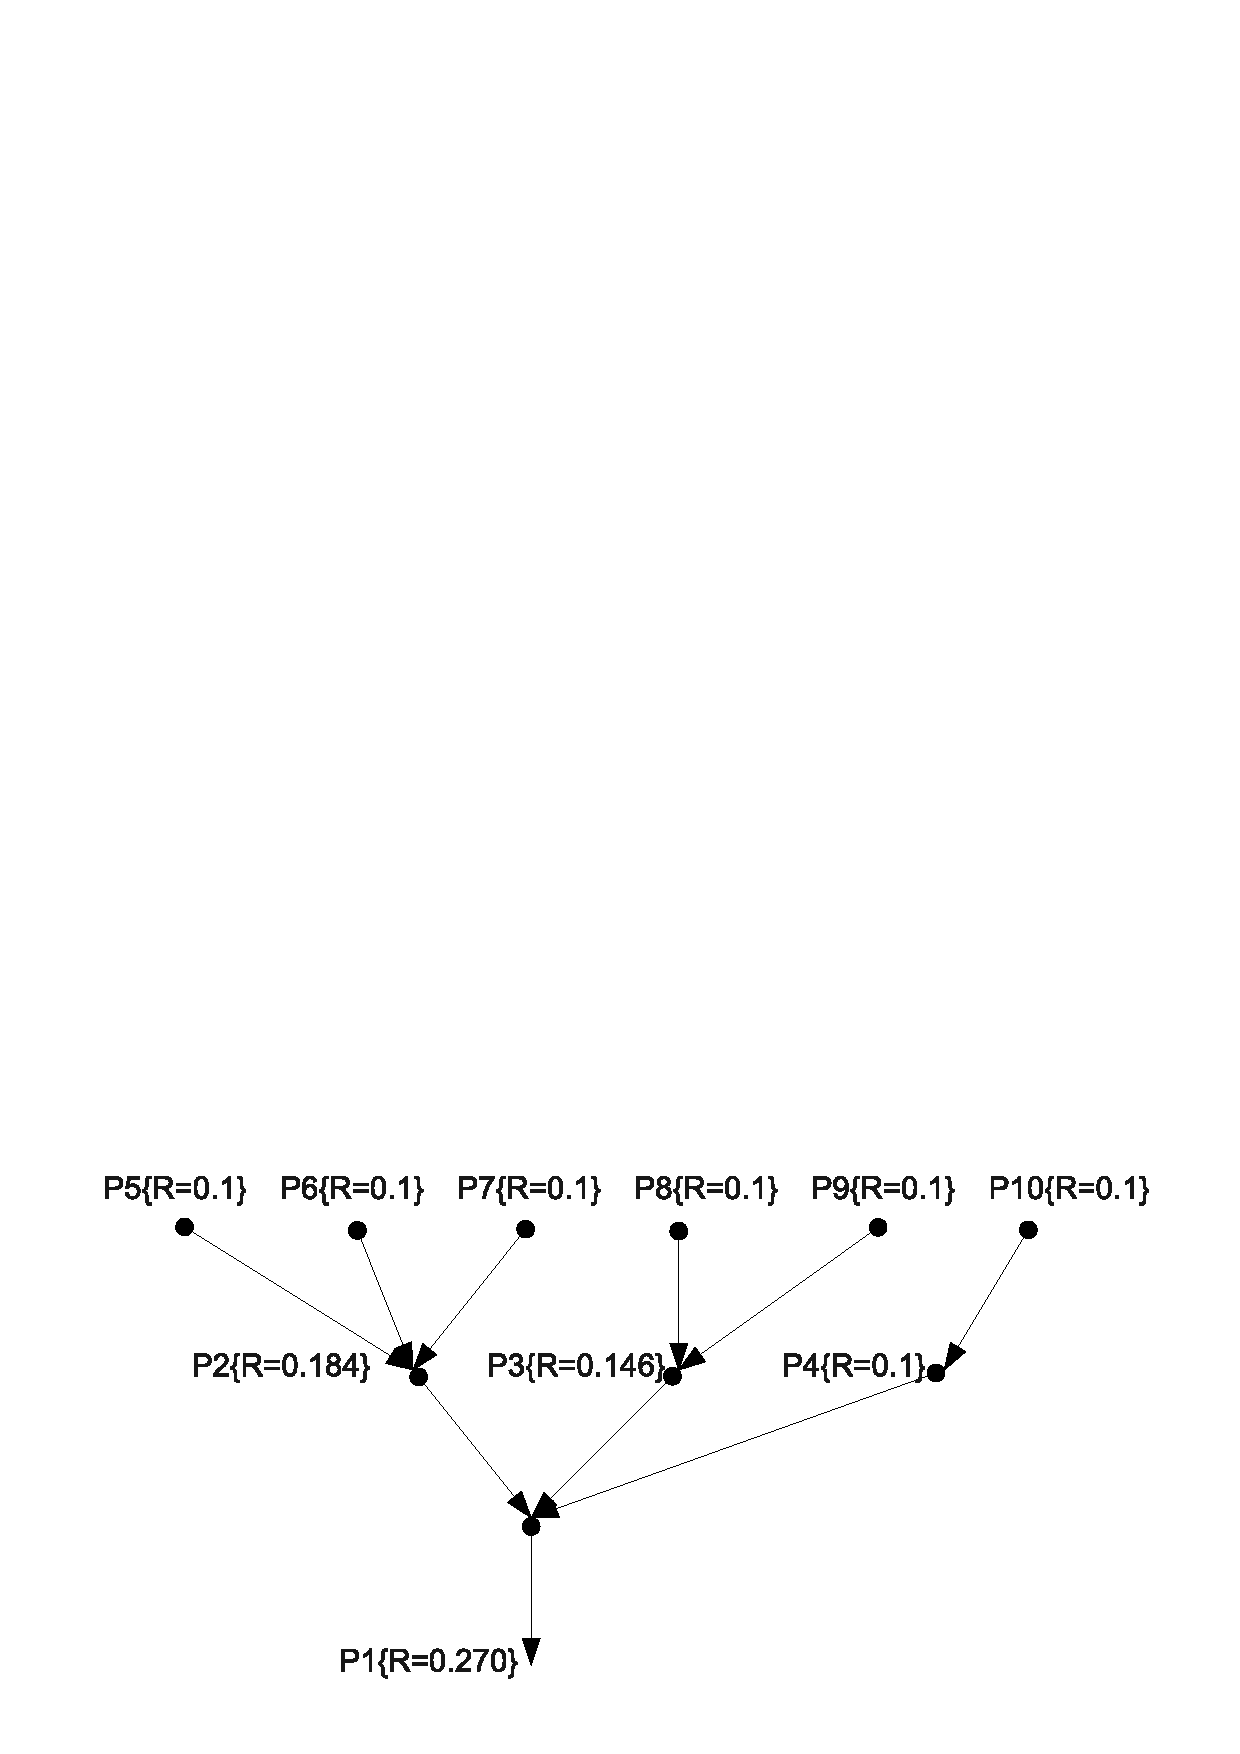
\includegraphics[width=130mm]{images/model/node_radius.pdf}
	\captionof{figure}{Obliczone promienie węzłów dla przykładowego drzewa.}
	\label{node_radius}
\end{center}


\begin{center}
	\includegraphics[width=130mm]{images/model/two_segments.png}
	\captionof{figure}{Dwa wyrenderowane segmenty wokół węzłów P1 i P2}
	\label{two_segments}
\end{center}

\subsection{Model gałęzi}
Dobrym przybliżeniem gałęzi jest uogólniony walec (ang. generalized cylinder). Jest to powierzchnia w przestrzeni $R^3$, której przekrój poprzeczny jest krzywą zamkniętą.

Gałąź jest reprezentowana przez listę kolejnych węzłów o największych średnicach idąc od dołu drzewa. Pozostałe węzły są początkami gałęzi potomnych. Przez połączenie ze sobą odpowiednich punktów z segmentów sąsiednich węzłów otrzymujemy uogólniony walec (rys. \ref{two_segments}).

Gałąź może być początkiem kolejnych konarów, dlatego posiada kolekcję gałęzi potomnych.

\begin{center}
	\includegraphics[width=130mm]{images/model/branching.png}
	\captionof{figure}{Fragment drzewa. Gałąź główna(kolor brązowy) w widocznym obszarze posiada 3 gałęzie potomne(kolor zielony).}
	\label{branching}
\end{center}
\subsection{Model liścia}
Liść cechuje się dwiema właściwościami: normalną do powierzchnii liścia oraz wektorem wyznaczającym kierunek liścia. Oba wektory są do siebie prostopadłe. Liść jest związany z konkretnym węzłem.

\begin{center}
	\includegraphics[width=80mm]{images/model/leaf_vects.png}
	\captionof{figure}{Liść z zaznaczonymi wektorami normalnym(zielony) i kierunkowym(czerwony). }
	\label{leaf_vect}
\end{center}

Wektor normalny jest wyznaczany na podstawie położenia liścia względem punktu (0,0,0). Dodatkowo jest obciążany wektorem grawitacji, którego współrzędna Z jest losowa z zakresu $\langle-0.9;0\rangle$. 



Liście są rozkładane są na gałęziach w sposób losowy, przy czym rozkład nie jest równomierny. Prawdopodobieństwo umiejscowienia liścia na końcu gałęzi jest znacznie większe niż na początku. Efekt ten uzyskaliśmy w następujący sposób: $node\_id = \lceil\sqrt{rand()}*(nodes\_length-1)\rceil$.

\begin{description}
	\item[node\_id] indeks węzła w danej gałęzi, do którego zostanie doczepiony liść
	\item[nodes\_length] jest liczbą węzłów należących do danej gałęzi.
	\item[rand()] zmienna losowa o rozkładzie równomiernym z zakresu $(0;1\rangle$
\end{description}

\subsection{Wygładzanie gałęzi przy pomocy algorytmu Chaikina \cite{smoothing}}
\subsubsection{Wstęp}
W 1974r. George Chaikin opublikował algorytm generowania krzywych ze skończonej liczby punktów kontrolnych. Algorytm ten okazał się bardzo interesujący przez niski stopień swojej komplikacji. Opiera się jedynie na ścinaniu wierzchołków początkowego wielokąta.

Tworzenie krzywej następuje iteracyjnie. Proces można można powtarzać, aż do osiągnięcia wymaganej rozdzielczości krzywej (rys. \ref{chaikin_1}).

\begin{center}
	\includegraphics[width=80mm]{images/model/chaikin_1.png}
	\captionof{figure}{Kolejne iteracje algorytmu Chaikina. \cite{smoothing}}
	\label{chaikin_1}
\end{center}

\subsubsection{Opis algorytmu}

Dla danego wielokąta \{$P_1$, $P_2$, ..., $P_n$\} wyznaczamy wielokąt pochodny \{$R_1$, $L_1$, $R_2$, $L_2$, ..., $R_n$, $L_n$\}, gdzie
$L_i = \frac{1}{4}P_{i-1} + \frac{3}{4}P_i$ oraz $R_i = \frac{3}{4}P_i + \frac{1}{4}P_{i+1}$.
Nowo powstały wielokąt składa się z $2n$ wierzchołków.

\begin{center}
	\begin{picture}(200,100)
		\put(10,10){\circle*{5}}
		\put(5,15){$P_{i-1}$}
	
		\put(90,70){\circle*{5}}
		\put(85,75){$P_i$}
	
		\put(190,20){\circle*{5}}
		\put(175,25){$P_{i+1}$}
	
		\put(10,10){\line(4,3){80}}
		\put(90,70){\line(2,-1){100}}
		
		\put(70,55){\circle*{5}}
		\put(65,60){$L_i$}
		\put(115,57.5){\circle*{5}}
		\put(110,62.5){$R_i$}
		
		\multiput(70,55)(10,0){5}{\line(1,0){5}}
		
	\end{picture}
	\captionof{figure}{Wierzchołki pochodne dla $P_i$.}
\end{center}

\subsubsection{Zastosowanie algorytmu Chaikina dla gałęzi}
Algorytm Chaikina w podstawowej wersji dla każdego punktu do wyznaczenia wierzchołków pochodnych, wymaga 2 sąsiadów. Chcąc zastosować wcześniej wspomnianą metodę dla gałęzi (łamana otwarta), trzeba wprowadzić pewne modyfikacje podczas przekształcania jej końców.


\begin{itemize}
	\item{Dla $i=1$ lub $i=n$: $L_i = R_i = P_i$}
	\item{Dla $i=2$: $L_i = \frac{1}{2}P_{i-1} + \frac{1}{2}P_i$ oraz $R_i = \frac{3}{4}P_i + \frac{1}{4}P_{i+1}$}
	\item{Dla $i=n-1$: $L_i = \frac{1}{4}P_{i-1} + \frac{3}{4}P_i$ oraz $R_i = \frac{1}{2}P_i + \frac{1}{2}P_{i+1}$}
	\item{Dla pozostałych przypadków: $L_i = \frac{1}{4}P_{i-1} + \frac{3}{4}P_i$ oraz $R_i = \frac{3}{4}P_i + \frac{1}{4}P_{i+1}$}
\end{itemize}

\begin{center}
	\includegraphics[width=130mm]{images/model/chaikin_branch.pdf}
	\captionof{figure}{Kolejne iteracje algorytmu Chaikina dla łamanej otwartej.}
	\label{chaikin_branch}
\end{center}

\subsection{Korona - TODO}
Algorytm kolonizacyjny w pierwszym kroku rozmieszcza atraktory wewnątrz danej podprzestrzenii, która to determinuje swoim kształtem wygląd wygenerowango drzewa. Wybór typu korony został ograniczony do 3 kształtów.
\begin{itemize}
	\item{sfera - możliwość zmiany promienia}
	\item{ścięty stożek - możliwość zmiany wysokości oraz promiania dolnej i górnej podstawy}
	\item{\textit{spline crown} - korona tworzona na skutek obrotu krzywej sklejalnej trzeciego stopnia wokół osi OX}
\end{itemize}

\begin{center}
	\includegraphics[width=130mm]{images/model/crowns.png}
	\captionof{figure}{Typy koron (sfera, ścięty stożek, \textit{spline crown})}
	\label{crowns}
\end{center}

\section{Teksturowanie}
Aplikacja obsługuje jedynie tekstury w formacie 24bit BMP. 
Ponadto wymiary tekstur w pikselach muszą być potęgą dwójki.
Dla tekstur liści aplikacja interpretuje kolor czarny jako ${100\%}$ przeźroczystość tekstury.

Ułożenie tekstury kory na pniu można regulować za pomocą parametrów:
\begin{itemize}
\item ${kx}$ -liczba tekstur potrzebna do owinięcia pnia
\item ${ky}$ - stosunek rozmiaru tekstury do odległości mierzonej wzdłuż pnia
\end{itemize}
Poniżej przedstawiono przykładowy fragment pnia drzewa utworzony dla ${kx=2}$ i ${ky=(0.2..0.5)}$
\begin{center}
	\includegraphics[width=140mm]{images/textures/ky.png}
	\captionof{figure}{Wpływ współczynnika ky na wygląd pnia. }
	\label{ky_texture}
\end{center}
Poniżej przedstawiono przykładowy fragment pnia drzewa utworzony dla ${ky=0.5}$ i ${kx=(1..4)}$
\begin{center}
	\includegraphics[width=140mm]{images/textures/kx.png}
	\captionof{figure}{Wpływ współczynnika kx na wygląd pnia. }
	\label{kx_texture}
\end{center}



\chapter{Dokumentacja}

\section{Diagramy klas}

\begin{center}
	\includegraphics[width=130mm]{images/treemaker_uml}
	\label{treemaker_uml}
\end{center}

\section{Eksport modelu}
Ponieważ format danych używany w programie nie jest zgodny z powszechnie uznanymi formatami modeli trójwymiarowych, aby zachować kompatybilność należy przeprowadzić eksport modelu do 
formatu zewnętrznego. Format .OBJ zgodnie wymaganiami jest obsługiwany przez program Blender.
Został on opracowany przez firmę Wavefront Technologies i ze względu na swoją prostotę stał się szybko
popularny wśród programów do obróbki grafiki trójwymiarowej. Na format składa się tekstowy z rozszerzeniem .obj 
zawierający opis geometrii obiektu, dodatkowo format przewiduje odwołanie do pliku z rozszerzeniem .mtl zawierającym
opis materiałów (kolorów i tekstur).


\subsection{Struktura pliku .obj}
Plik jest podzielony na linie, z czego każda linia moze zawierać:
\begin{itemize}
\item '\#' : komentarz 
\item mtllib [nazwa pliku .mtl] :odwołanie do pliku z materiałami
\item usemtl [nazwa materiału]  :nakaz uzycia materiału
\item o [nazwa obiektu]         :definicję obiektu
\item g [nazwa grupy]           :definicję grupy: 
\item v [x] [y] [z]             :współrzędne wierzchołka
\item vn [x] [y] [z]            :współrzędne wektora normalnego
\item vt [x] [y]                :współrzędne tekstury
\item f [v1/vn1/vt1] [v2/vn2/vt2] [v3/vn3/vt3] :definicja trójkąta 
\end{itemize}
Warto nadmienić, iż przy definiowaniu trójkątów podajemy indeksy (numerowane od 1) poszczególnych współrzędnych w znajdujących się w pliku.
Istotne jest również to, iż współrzędne tekstury i wektora normalnego trójkąta są opcjonalne, a sam wektor normalny może być odtworzony poprawnie,
nawet jeśli nie został zawarty w pliku dzięki podaniu współrzędnych wierzchołków zgodnie z ruchem wskazówek zegara.


\subsection{Struktura pliku .mtl}
Plik .mtl może zawierać definicje wielu materiałów. Podobnie jak plik .obj jest to plik tekstowy z informacjami znajdującymi
się w kolejnych liniach mogących zawierać:
\begin{itemize}
\item '\#' : komentarz 
\item newmtl [nazwa materiału]: definicja materiału
\item Ka [r] [g] [b]: ambient kolor
\item Kd [r] [g] [b]: diffuse kolor
\item Ks [r] [g] [b]: specular kolorów
\item Ns [x]        : specular cooef
\item d  [x]        : przezroczystosc
\item map\_Ka [nazwa pliku]: tekstura 
\end{itemize}


\subsection{Procedura eksportu}
Model drzewa jest eksportowany w dwóch etapach, jako dwie osobne grupy jednego obiektu. Pierwszą grupę stanowi pień drzewa, drugą natomiast jego liście.
Pozwala to na użycie różnych tekstur dla tych elementów drzewa. Program grupuje współrzędne wierzchołków i tekstur by zmniejszyć rozmiar tworzonego pliku, a następnie
zapisuje je do pliku \{models/tree0.obj\}. Dodatkowo program tworzy plik \{models/tree0.mtl\} zawierający opis materiałów i ścieżki do tekstur. 
\section{Opis interfejsu użytkownika}

\subsection{Okno główne}
\includegraphics[width=120mm]{images/gui/main_window.png}
\begin{enumerate}
	\item {Podgląd wygenerowanego drzewa.}
	\item {Toolbar.}
	\item {Panel z ustawieniami generatora.}
\end{enumerate}

\subsection{Podgląd wygenerowanego modelu}
\includegraphics[width=120mm]{images/gui/model_view.png}
\begin{enumerate}
	\item {Siatka wyznaczająca poziom ziemi.}
	\item {Układ współrzędnych.}
	\item {Model drzewa.}
	\item {Aktywna korona.}
	\item {Nieaktywna korona.}
\end{enumerate}

\subsection{Toolbar}
\includegraphics[width=50mm]{images/gui/toolbar.png}
\begin{enumerate}
	\item {Resetuj konfigurację.}
	\item {Wczytaj konfigurację.}
	\item {Zapisz konfigurację.}
	\item {Generuj nowy model.}
	\item {Odśwież model.}
	\item {Eksportuj model.}
\end{enumerate}

\subsection{Opcje algorytmu}
\begin{tabular}{lr}
\parbox[b]{95mm}{
\begin{enumerate}
	\item {Wybór algorytmu generującego drzewo.}
	\item {Ziarno generatora pseudo-losowego.}
	\item {Odległość pomiędzy sąsiednimi węzłami w drzewie.}
	\item {Liczba atraktorów, z których generowane jest drzewo.}
	\item {Influence distance - promień przyciągania atraktorów do drzewa.}
	\item {Kill distance - ?.}
\end{enumerate}
} &
\includegraphics[width=35mm]{images/gui/algorithms_panel.png} \\
\end{tabular}



\subsection{Opcje korony}
\begin{tabular}{lr}
\parbox[b]{95mm}{
\begin{enumerate}
	\item {Typ korony (sfera, ścięty stożek, bryła obrotowa oparta o krzywą sklejalną trzeciego stopnia).}
	\item {Dodaj koronę.}
	\item {Lista dodanych koron.}
	\item {Współrzędna X wybranej korony.}
	\item {Współrzędna Y wybranej korony.}
	\item {Współrzędna Z wybranej korony.}
	\item {TODO widok dla każdego typu korony}
\end{enumerate}
} &
\includegraphics[width=35mm]{images/gui/crown_panel.png} \\
\end{tabular}


\subsection{Opcje wyświetlania}
\begin{tabular}{lr}
\parbox[b]{95mm}{
\begin{enumerate}
	\item {Wyświetla dodane korony.}
	\item {Wyświetla liście.}
	\item {Wyświetla korę.}
	\item {Wyświetla trawę.}
\end{enumerate}
} &
\includegraphics[width=35mm]{images/gui/rendering_panel.png}\\
\end{tabular}

\subsection{Opcje pnia}
\begin{tabular}{lr}
\parbox[b]{95mm}{
\begin{enumerate}
	\item {Współczynnik $radius factor$. Wpływa na grubość pnia przy łączeniu gałęzi.}
	\item {Współczynnik $a$.}
	\item {Współczynnik $m$.}
	\item {Liczba punktów tworzących segment.}
	\item {Liczba tekstur potrzebną do owinięcia pnia.}
	\item {Stosunek rozmiaru tekstury do odległości mierzonej wzdłuż pnia.}
\end{enumerate}
} &
\includegraphics[width=35mm]{images/gui/trunk_panel.png}\\
\end{tabular}

\subsection{Opcje liści}
\begin{tabular}{lr}
\parbox[b]{95mm}{
\begin{enumerate}
	\item {Liczba liści doczepianych do wygenerowanego modelu.}
	\item {Lista rodzajów liści.}
	\item {Rozmiar danego liścia.}
	\item {?}
	\item {Współczynnik wpływający na liczbę liści danego typu.}
	\item {Dodawanie nowego typu liścia.}
\end{enumerate}
} &
\includegraphics[width=35mm]{images/gui/leaves_panel.png}\\
\end{tabular}




\subsection{Edytor}
\begin{tabular}{lr}
\parbox[b]{95mm}{
\begin{enumerate}
	\item {Tryb zaznaczania gałęzi - odpowiednio: cała gałęź, od punktu do końca gałęzi oraz od punktu do punktu}
	\item {Zastosuj dla wszystkich dzieci - edycji podlegają też gałęzie wychodzące z edytowanego fragmentu}
	\item {Przycinanie gałęzi}
	\item {Wygładzanie gałęzi (zwiększana jest rozdzielczość gałęzi)}
	\item {Zmniejszanie gałęzi}
	\item {Dociążanie gałęzi}
	\item {Działanie przeciwne do opcji 6}
\end{enumerate}
} &
\includegraphics[width=35mm]{images/gui/editor_panel.png} \\
\end{tabular}

\section{Kompilacja projektu}
\subsection{Wymagane biblioteki}
Zgodnie z wymaganiami programi powinien posiadać możliwie małą ilość zależności. System powinien posiadać kompilator GCC oraz bibliotekę GTK+ z rozszerzeniem do obsługi OpenGL.
Poniżej przedstawiono dokładne wersje bibliotek wymagane przez program.
\begin{itemize}
\item GTK+ 2.2
\item GTKGLEXT 1.2
\item MESA 7.8
\item GCC 4.4.4
\end{itemize}
\subsection{Uruchomienie}
Źródła programu zostały załączone na płycie CD, ponadto znajdują się na stronie https://code.google.com/p/treemaker/source/browse/.\\
Po ich pobraniu wystarczy wydać polecenie make w katalogu ze źródłami by rozpocząć kompilację programu. Jeśli przebiegła ona pomyślnie został utworzony
program wykonywalny o nazwie treemaker.



\chapter{Rezultaty}


\section{Testy wydajnościowe}
Po zakończeniu projektu przeprowadzono testy wydajnościowe aplikacji. Czas działania jednej iteracji naszej implementacji algorytmu kolonizacyjnego jest równy ${\Theta(n_i*m_i)}$, gdzie ${n_i}$ to liczba atraktorów
w danej iteracji, a ${m_i}$ to liczba węzłów w danej iteracji. Wynika on z konieczności wyznaczenia dla każdego atraktora najbliższego węzła drzewa.
Ciężko jest określić liczbę iteracji algorytmu potrzebnych do zakończenia, gdyż zależy ona równocześnie od kilku parametrów algorytmu.
 Na wykresie widzimy
szybki początkowy wzrost czasu potrzebnego na wygenerowanie modelu, a następnie zmianę szybkości wzrostu. Wynika ona z ograniczonej ilości
pamięci dostępnej dla procedury generowania, ustalonej by czas generowania drzewa dla dowolnej liczby atraktorów nie przekroczył kilkunastu sekund.



\begin{center}
	\includegraphics[width=90mm]{images/performance.pdf}
	\captionof{figure}{Czas generowania modelu w zależności od liczby atraktorów.}
\end{center}

\section{Ostateczny wygląd aplikacji}
\begin{center}
	\includegraphics[width=120mm]{images/gui/all.png}
	\captionof{figure}{Wygląd aplikacji.}
\end{center}

\section{Przykładowe modele drzew}
Poniżej przedstawiono przykładowe modele drzew, wraz z opisem głównych parametrów wpływających na ich ostateczny wygląd.
Wszystkie obrazy zostały utworzone przez program Blender. Więcej uzyskanych obrazów znajduje się na dołączonej płycie CD.
\begin{center}
	\includegraphics[width=100mm]{images/renders/greentree.png}
	\captionof{figure}{Wpływ liczby liści na wygląd drzewa}
\end{center}

\begin{center}
	\includegraphics[width=120mm]{images/renders/points.png}
	\captionof{figure}{Wpływ liczby atraktorów na wygląd drzewa}
\end{center}

\begin{center}
	\includegraphics[width=120mm]{images/renders/shape.png}
	\captionof{figure}{Wpływ kształtu korony na wygląd drzewa}
\end{center}

\begin{center}
	\includegraphics[width=120mm]{images/renders/smooth.png}
	\captionof{figure}{Wpływ wygładzania gałęzi na wygląd drzewa}
\end{center}




\chapter{Podsumowanie}

Celem naszego projektu inżynierskiego było stworzenie narzędzia do generowania trójwymiarowych modeli drzew. Rezultaty pracy pokrywają w 100\% cele postawione na początku. Wszystkie prace zostały wykonane zgodnie z harmonogramem oraz podziałem zadań.

Sukcesywnie podczas realizacji projektu pojawiało się coraz więcej nowych pomysłów na rozwój aplikacji.

Możliwości rozwoju:
\begin{my_itemize}
	%\item dodatkowe formaty obsługiwane przez eksporter
	\item model fizyczny drzewa
	%\item optymalizacja metod generowania drzewa
	\item dodanie nowych modyfikatorów wpływających na generowany model
	%\item generowanie korzenia
	\item generowanie liści oraz kory
	%\item generowanie kwiatów i owoców
	\item tworzenie kilku modeli kolonizujących tę samą przestrzeń jednocześnie - efekt współzawodniczenia o przestrzeń
	\item poprawienie edytora - dodanie kolejnych możliwości edycji
	\item ustawianie liści do światła
	\item dodanie opcji cofnij/powtórz podczas modyfikowania
	%\item kilkustopniowe generowanie
	%\item w środku drzewa zwykle nie ma liści
	\item inne algorytmy generowania - uwzględniające np. oświetlenie, wpływ wiatru
	%\item animacja wzrostu drzewa
	%\item malowanie "pędzlem" kory, np. dodawanie mchu
	\item optymalizacja modelu pod względem liczby wielokątów
	\item operacje logiczne na koronach
	\item wczytywanie koron z pliku xml
	\item generowanie dowolnej liczby drzew na podstawie pliku xml
	%\item zapisywanie ustawień do xml
	\item inne formaty tekstur niż bmp24bit
	\item filtry kolorów do tekstur
	\item zmienna geometria liści
\end{my_itemize}


\chapter*{Załączniki}
\begin{itemize}
	\item źródła programu dostępne na płycie CD, bądź pod adresem\\
	\textit{http://code.google.com/p/treemaker/source/browse/}
	\item screencast.avi - zrzut z ekranu demonstrujący użycie programu
\end{itemize}



% Literatura
\addcontentsline{toc}{chapter}{Bibliografia}
\begin{thebibliography}{1}
\bibitem{jankowski} M. Jankowski  \emph{Elementy grafiki komputerowej}. WNT 2006
\bibitem{spaceColonization} A. Runions, B. Lane, P. Prusinkiewicz: \emph{Modeling Trees with a Space Colonization Algorithm}.
Eurographics Workshop on Natural Phenomena 2007
\bibitem{particleMethod} Y. Rodkaew, P. Chongstitvatana, S. Siripant, C. Lursinsap \emph{Particle systems for plant modeling}. Plant growth modeling and applications. Proceedings of PMA03, pp. 210-217

\bibitem{honda} H. Honda \emph{Description of the form of trees by the parameters of the tree-like body: Effects of the branching angle and the branch length on the shape of th tree-like body}. Journal of Theoretical Biology 31 (1971), pp. 331-338
\bibitem{ulam} S. Ulam \emph{On some mathematical properties connected with patterns of growth on figures}. Proceedings of Symposia on Applied Mathematics 14 (1962), pp. 215-224
\bibitem{bloomenthal}J. Bloomenthal: \emph{Modeling the Mighty Maple}. SIGGRAPH '85 Proceedings of the 12th annual conference on Computer graphics and interactive techniques 1985
\bibitem{smoothing} P. Prusinkiewicz, F. Samavati, C. Smith, R. Karwowski:\emph{L-system description of subdivision curves}. International Journal of Shape Modeling 9 (1), pp. 41-59
\end{thebibliography}




\end{document}
